\appendix
\setcounter{chapter}{1}
\chapter{System UI and Training}
\renewcommand{\thefigure}{B.\arabic{figure}}
\bigskip
\bigskip
\medskip
{\large This section includes the images of the system UI and Training.}

\newpage
\begin{figure}[ht]
    \centering
    
\includegraphics[width=0.9\textwidth,height=0.4\textheight,keepaspectratio]{figures/Game_Menu.png}
    \caption{ Game Menu}
    \label{fig:System_UI_1}
\end{figure}

\begin{figure}[ht]
    \centering
    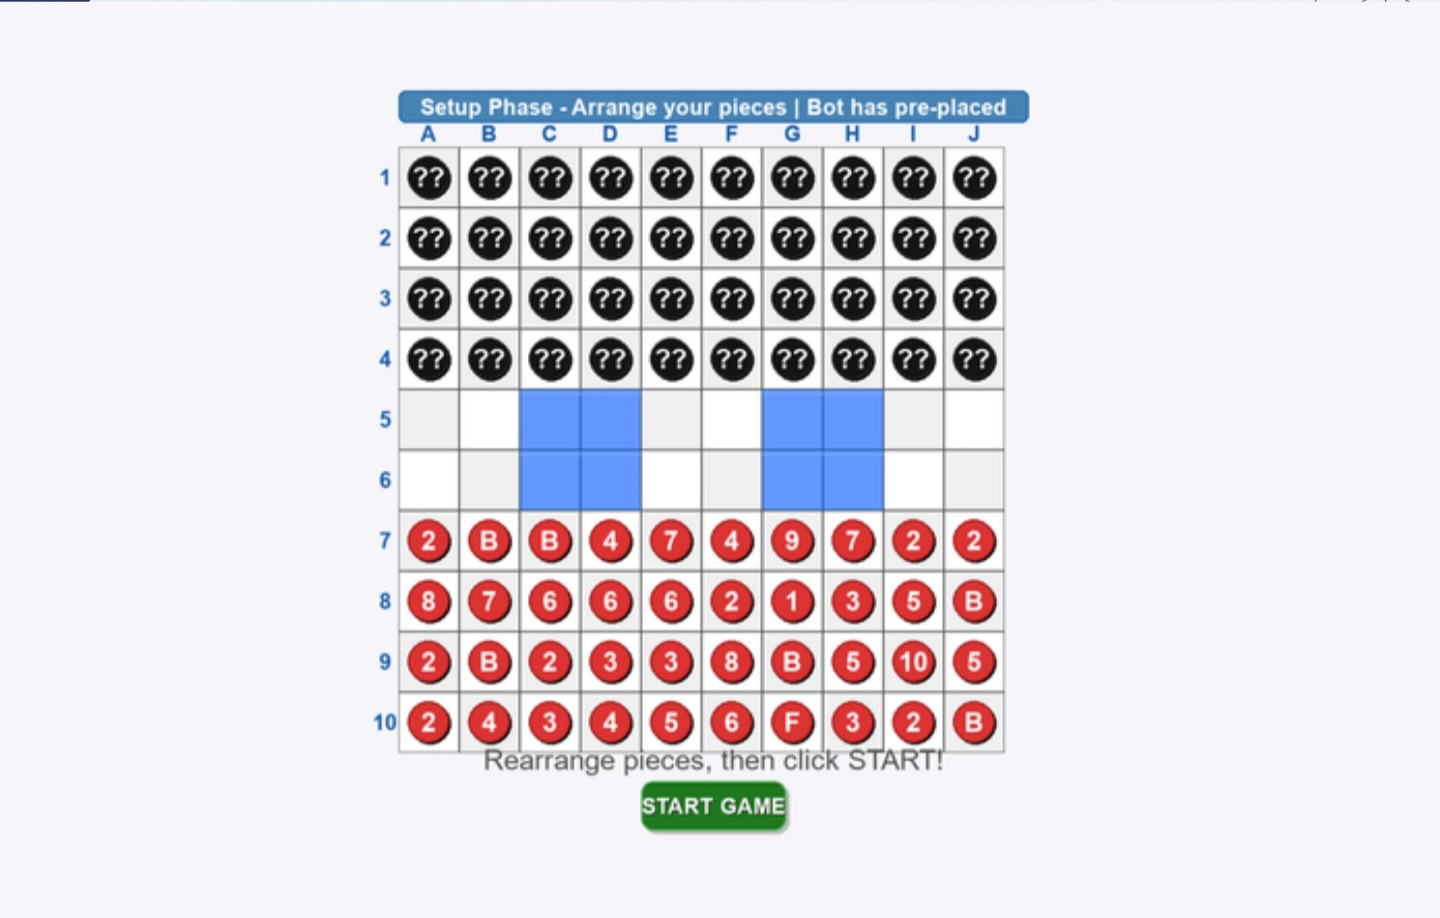
\includegraphics[width=0.9\textwidth,height=0.4\textheight,keepaspectratio]{figures/Arrange.png}
    \caption{Setup Phase}
    \label{fig:System_UI_2}
\end{figure}

\begin{figure}[ht]
    \centering
    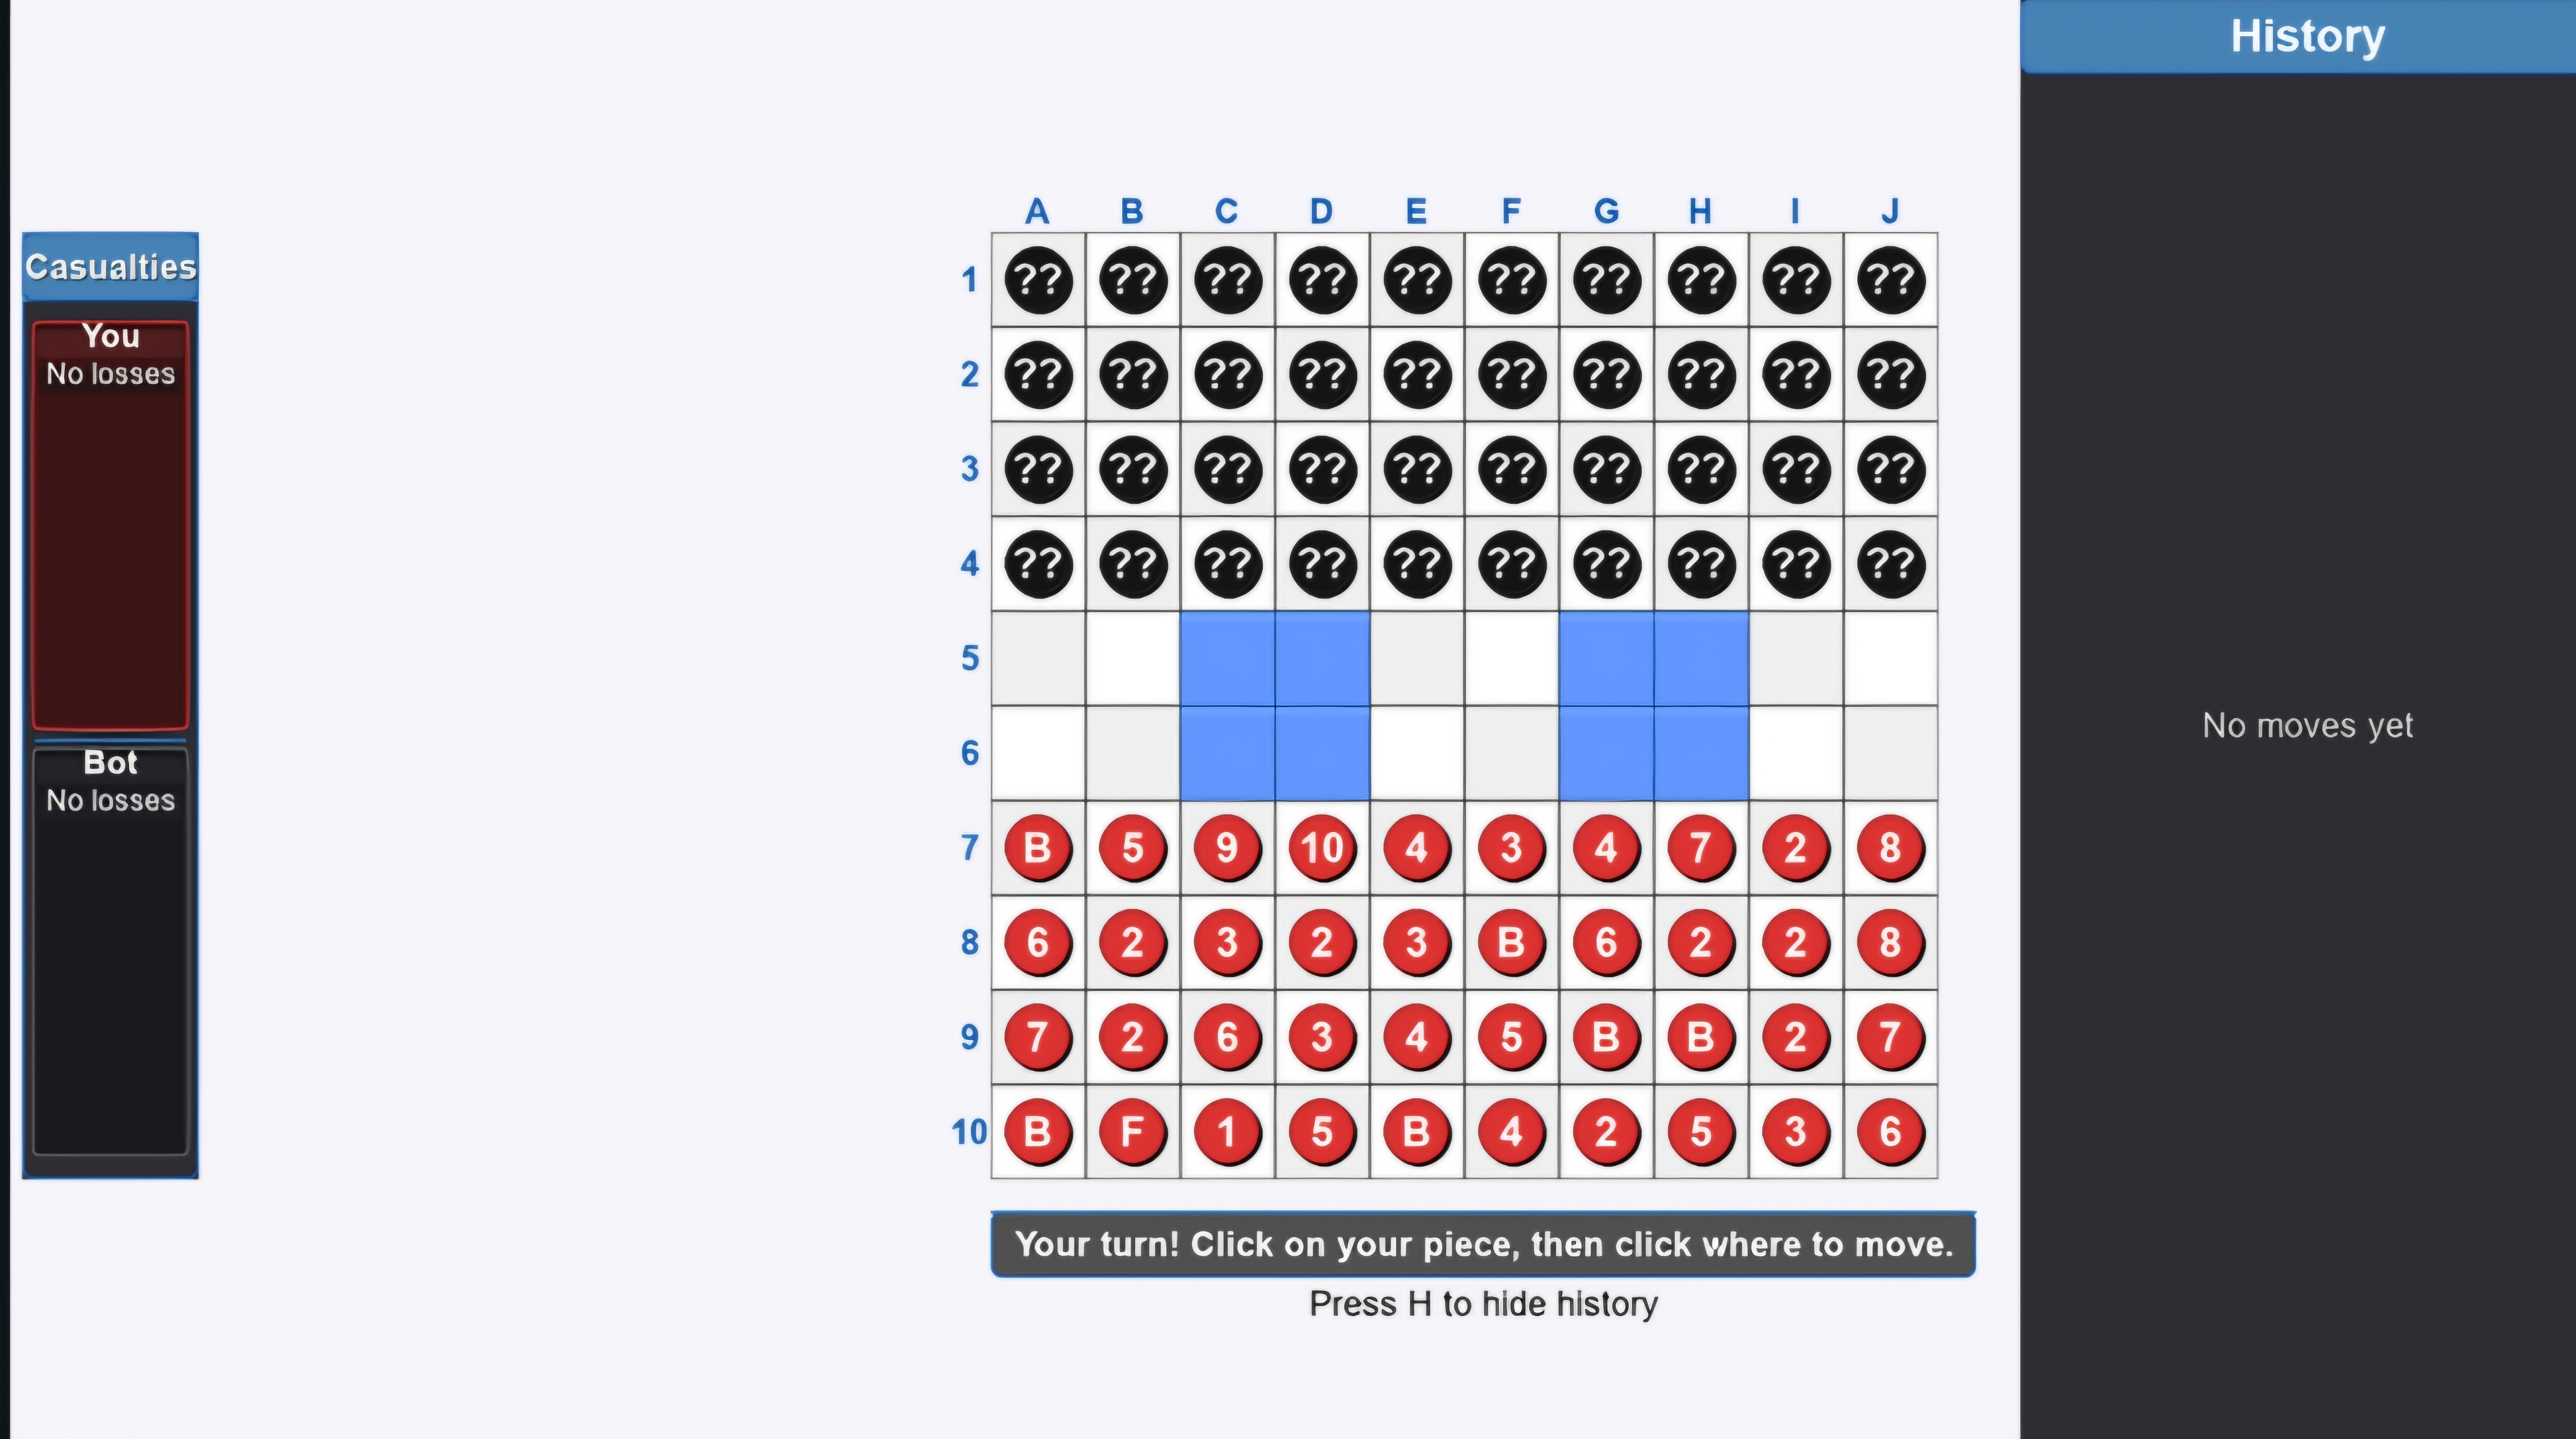
\includegraphics[width=0.9\textwidth,height=0.4\textheight,keepaspectratio]{figures/Game_Start.png}
    \caption{Game Start}
    \label{fig:System_UI_3}
\end{figure}

\begin{figure}[ht]
    \centering
    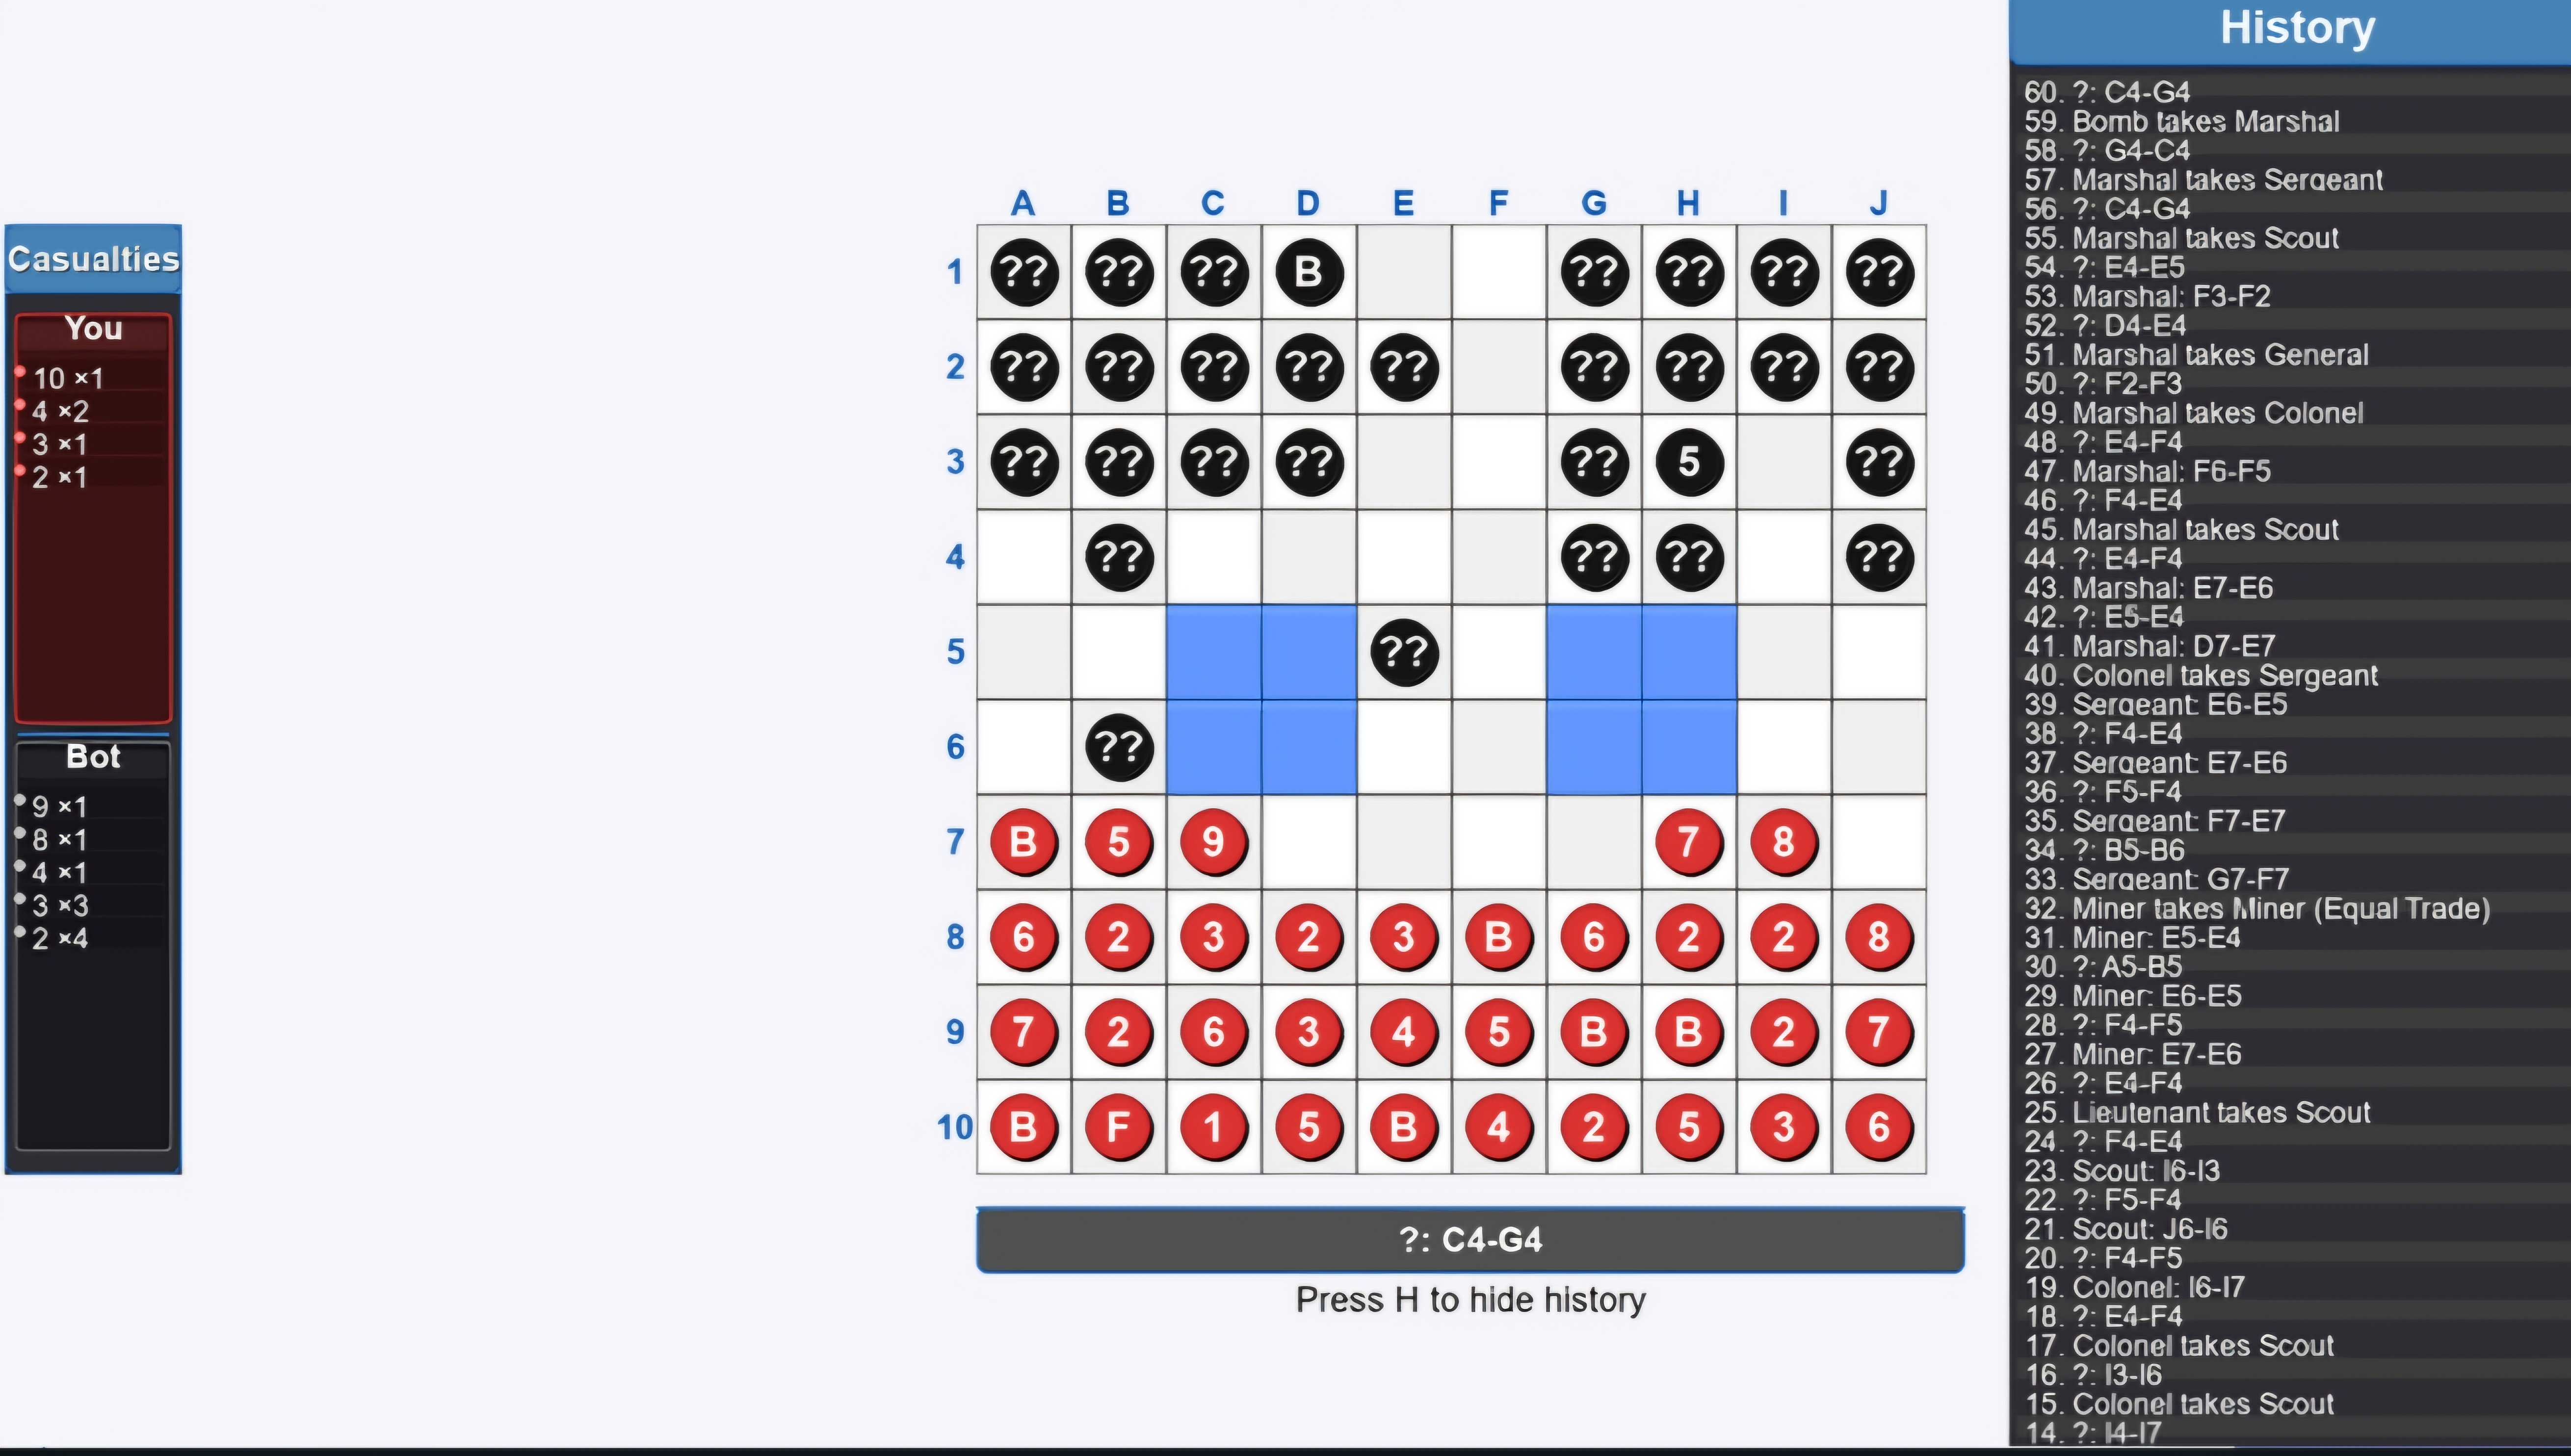
\includegraphics[width=0.9\textwidth,height=0.4\textheight,keepaspectratio]{figures/GameHistory.png}
    \caption{Battle and History}
    \label{fig:System_UI_4}
\end{figure}


\begin{figure}[ht]
    \centering
    
\includegraphics[width=0.9\textwidth,height=0.4\textheight,keepaspectratio]{figures/Victory.png}
    \caption{Victory Screen}
    \label{fig:System_UI_5}
\end{figure}


\begin{figure}[ht]
    \centering
    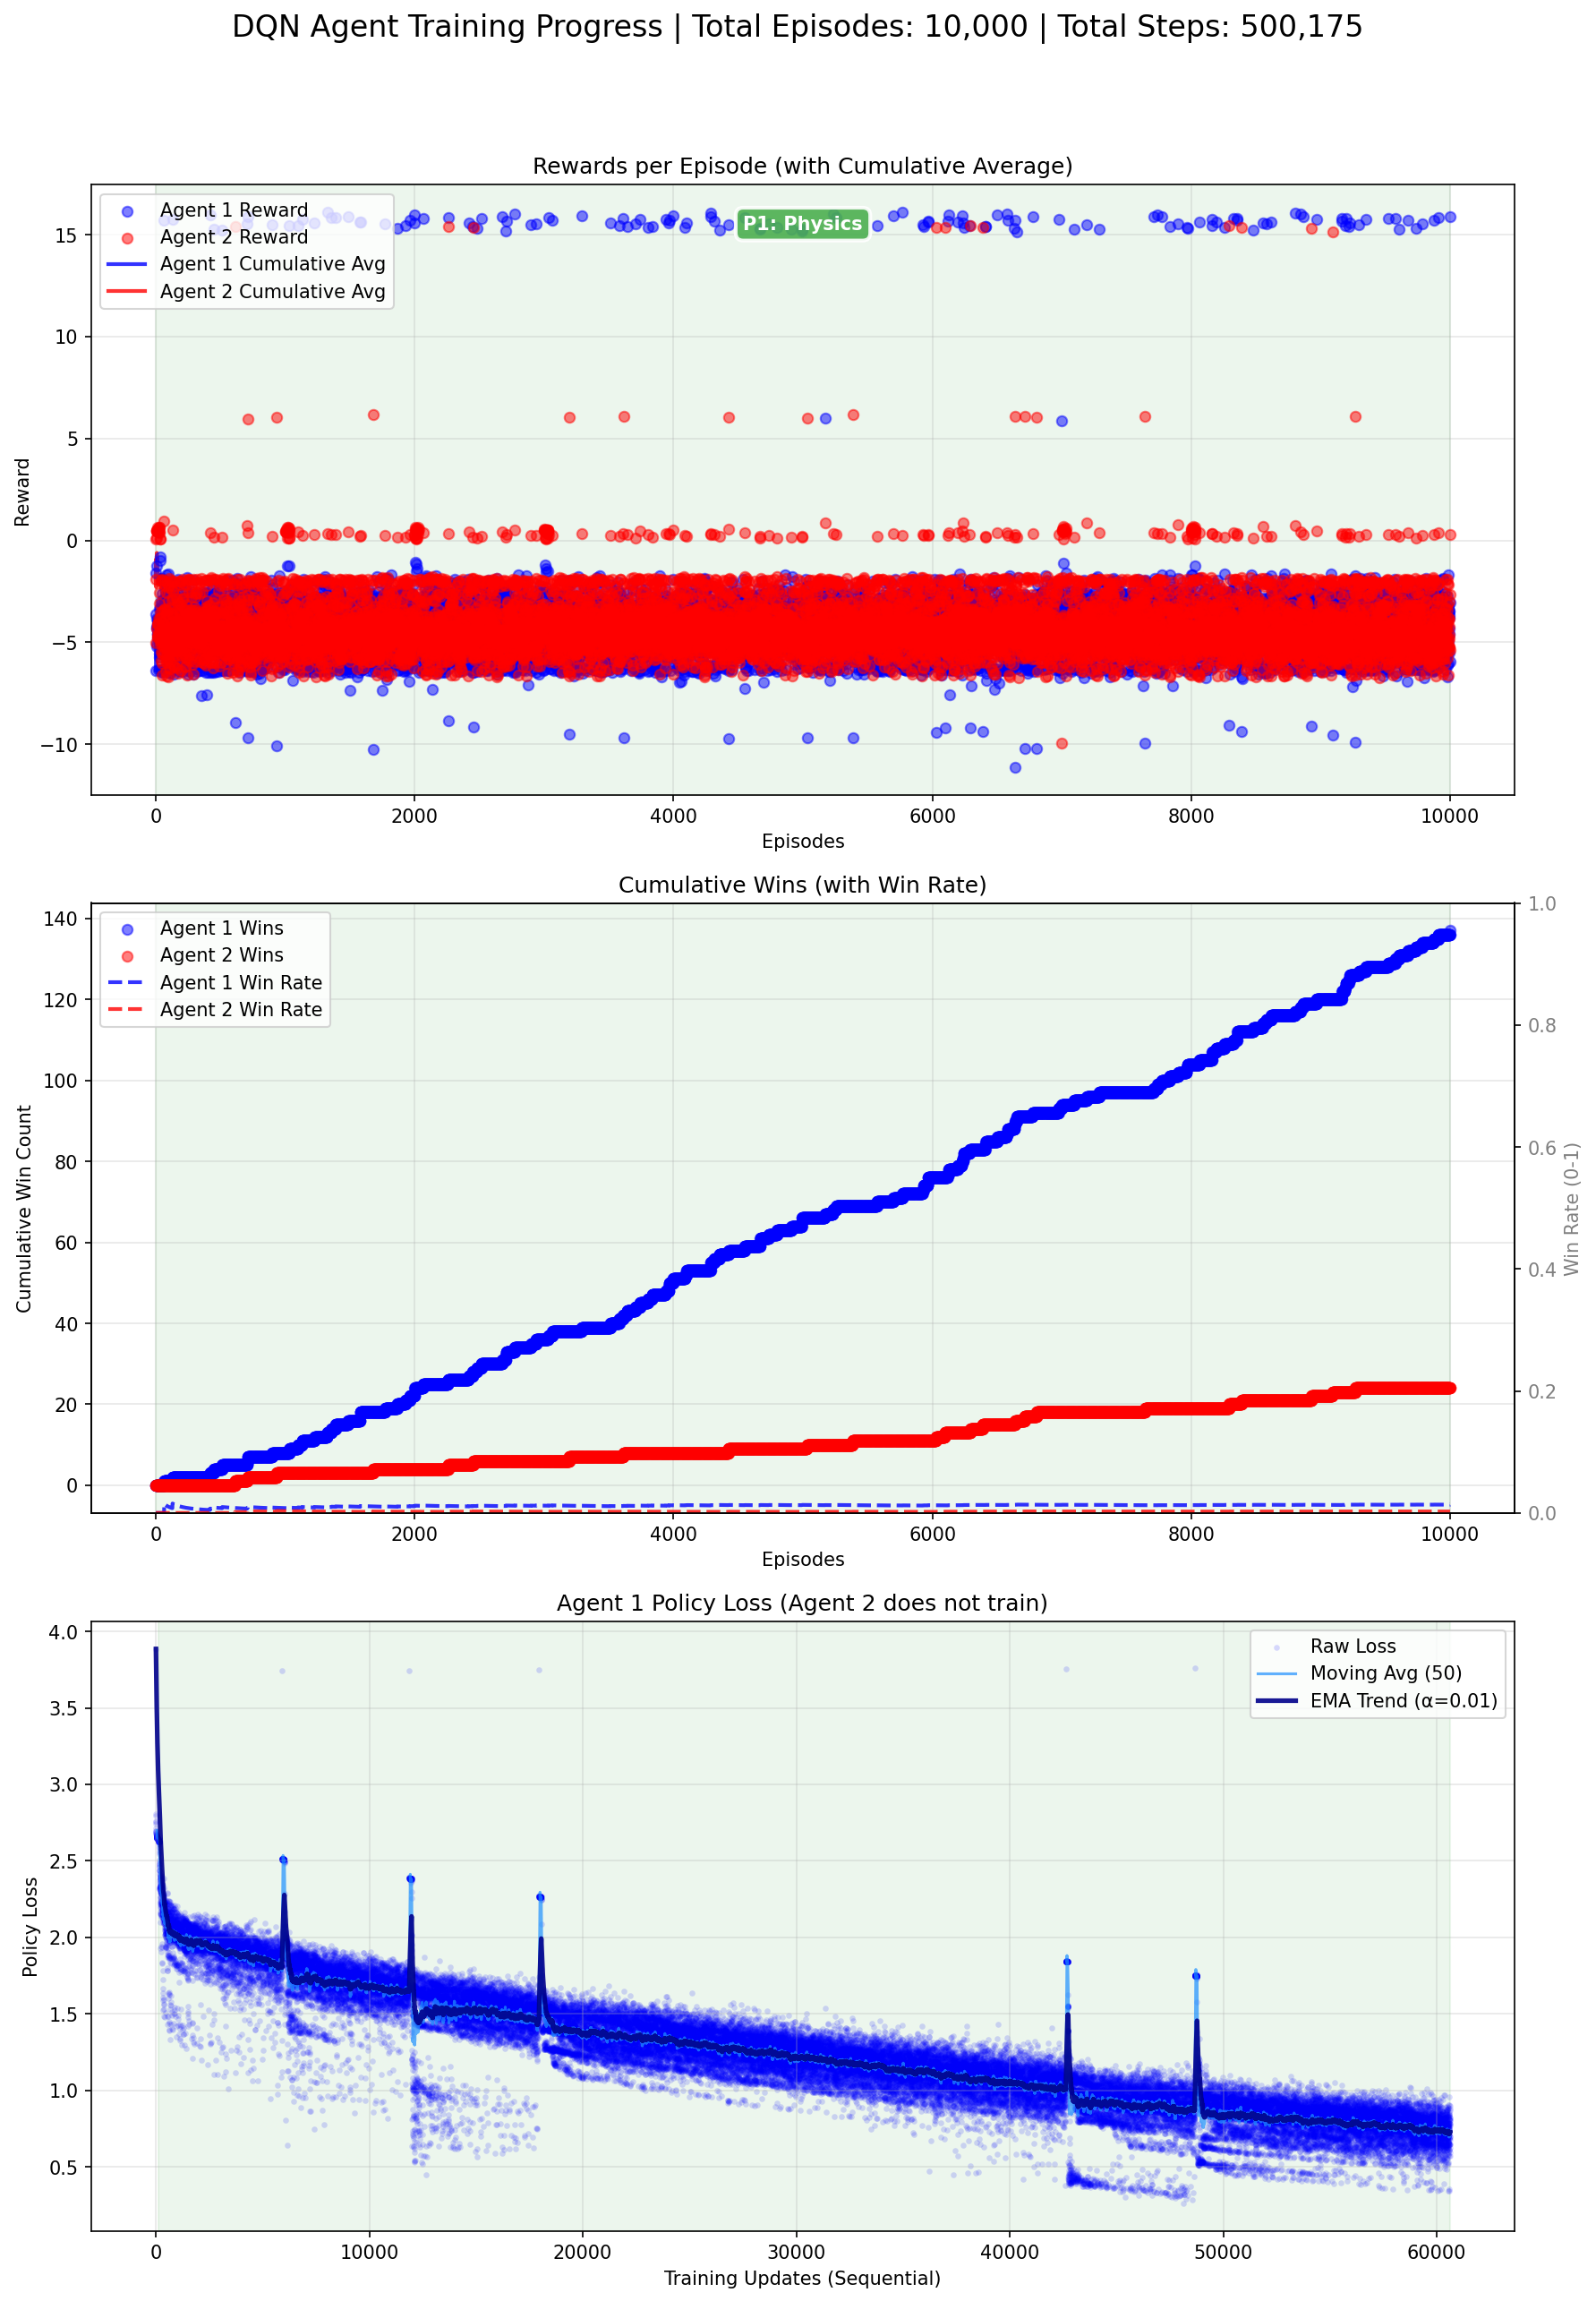
\includegraphics[width=0.9\textwidth,height=0.25\textheight,keepaspectratio]{figures/Results/training_progress_episode_10000.png}
    \caption{Training Progress: Episode 10,000}
    \label{fig:train_10k}
\end{figure}

\begin{figure}[ht]
    \centering
    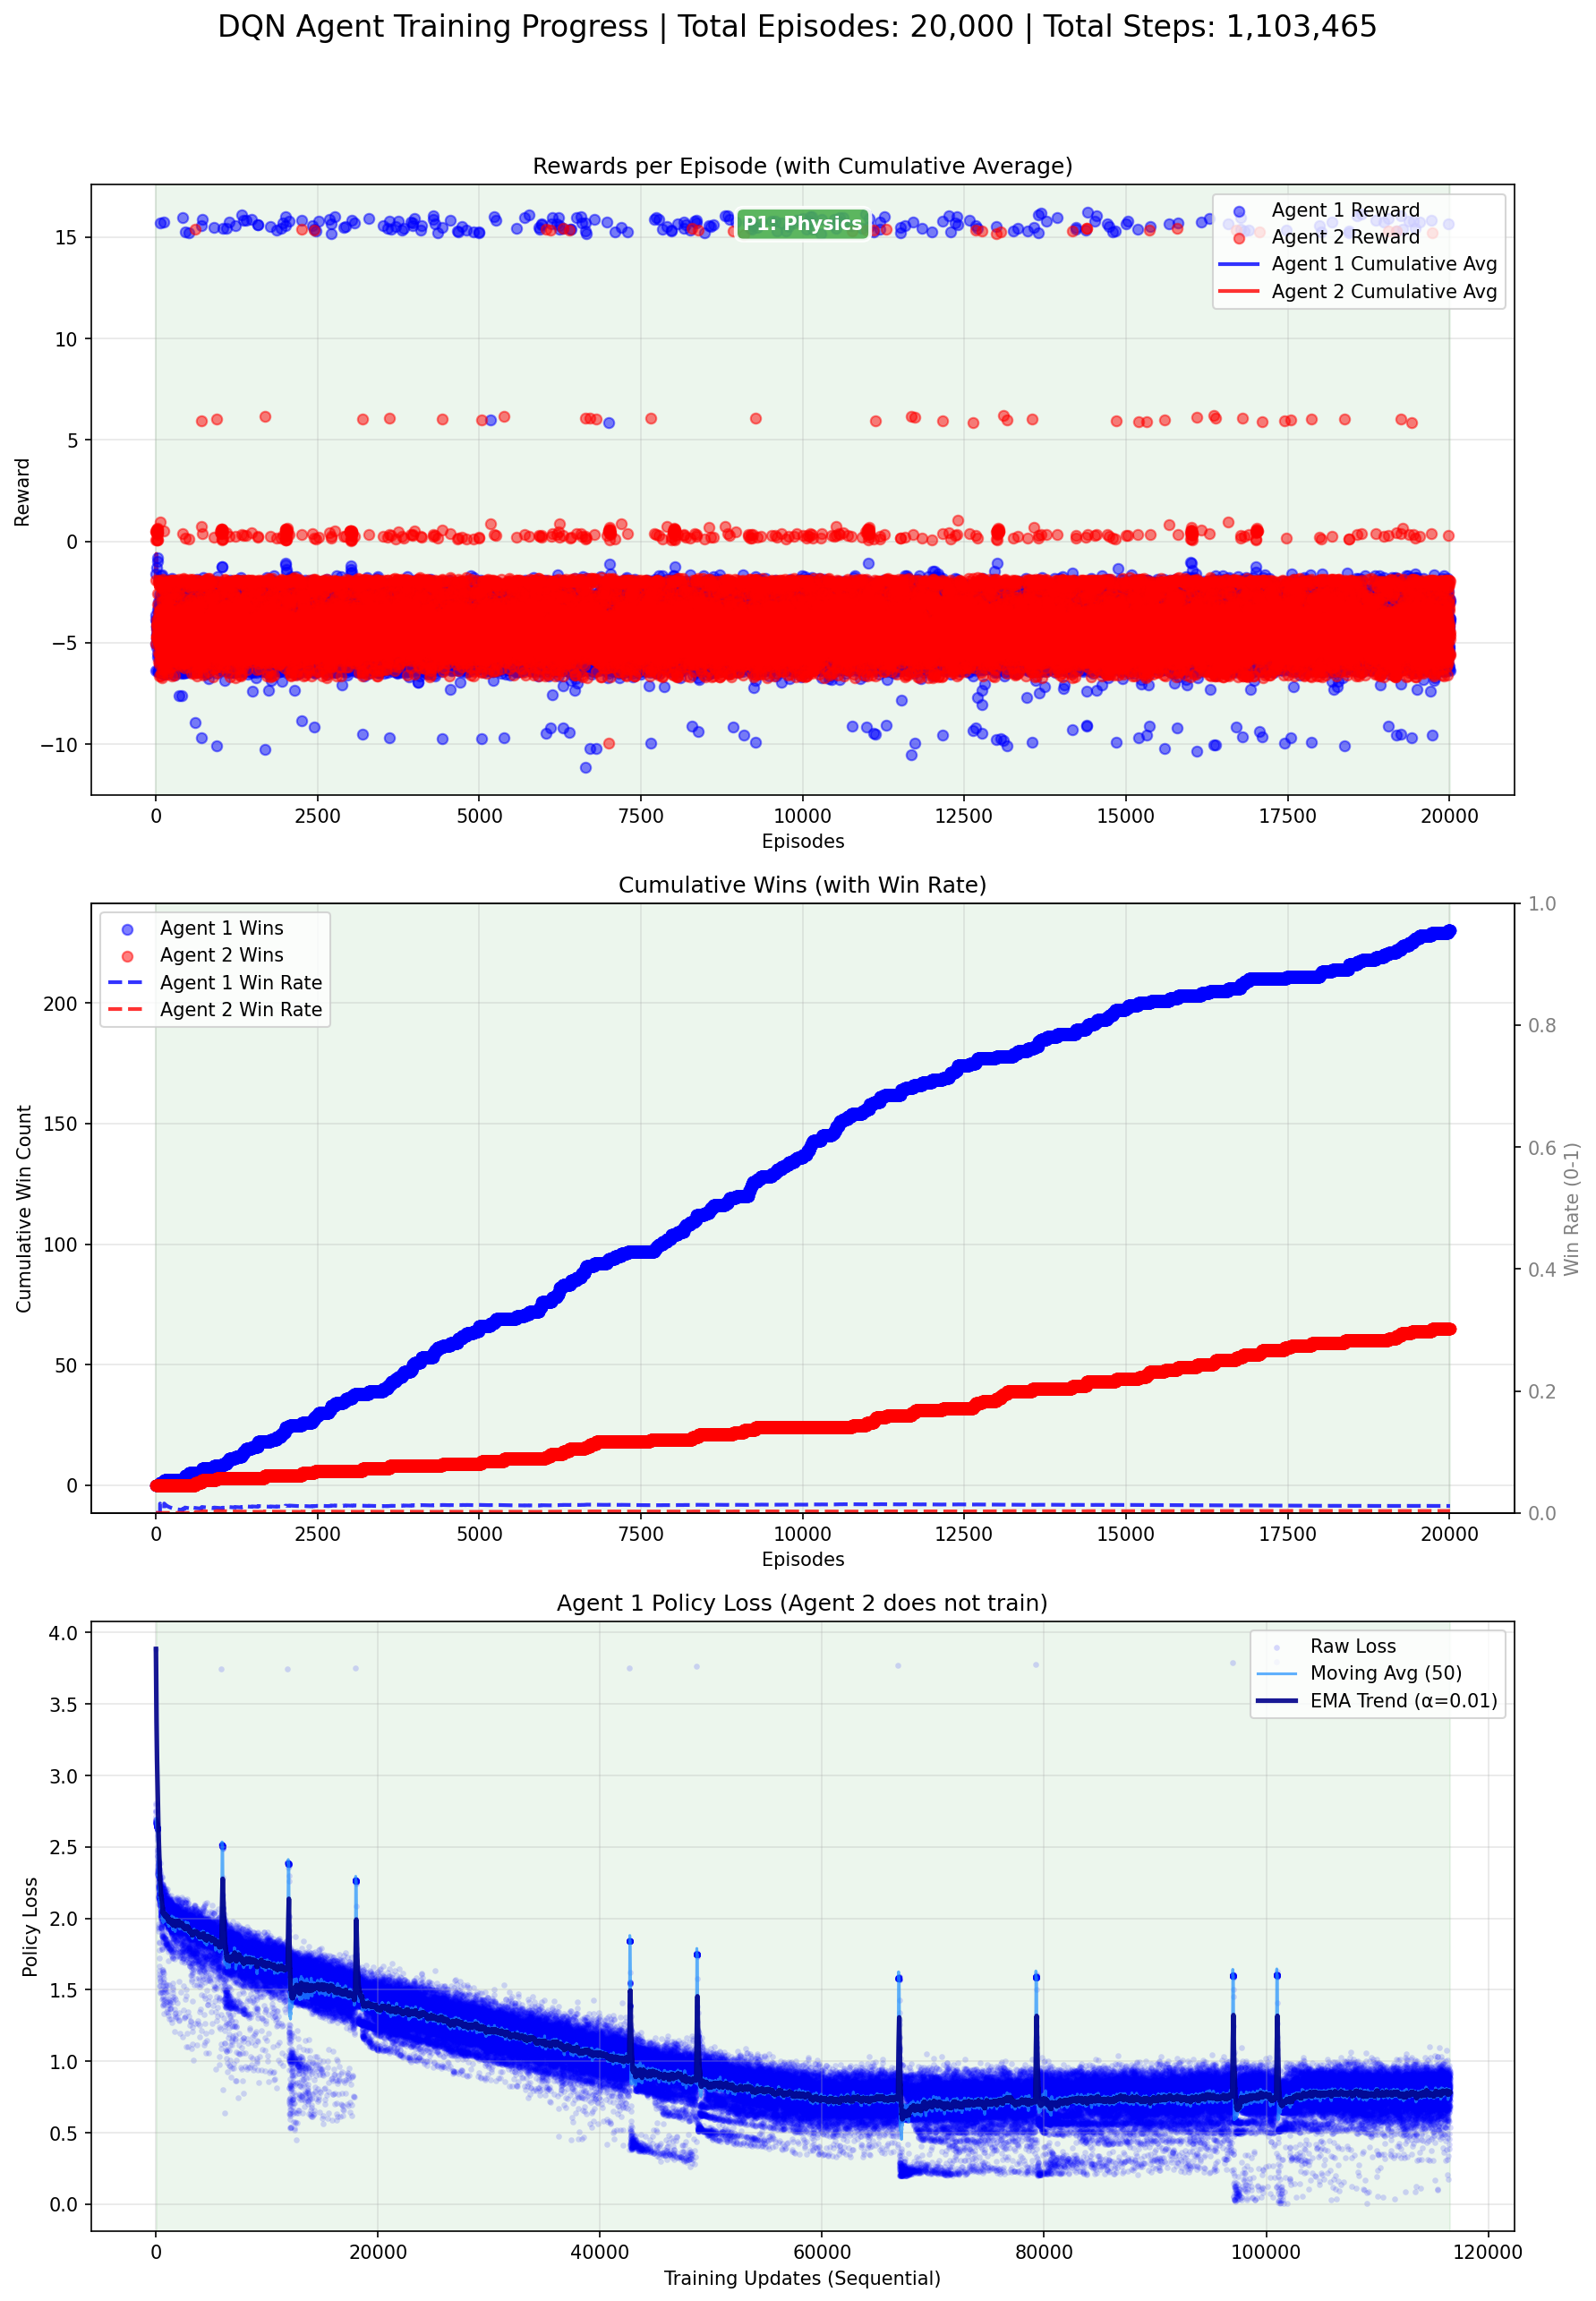
\includegraphics[width=0.9\textwidth,height=0.25\textheight,keepaspectratio]{figures/Results/training_progress_episode_20000.png}
    \caption{Training Progress: Episode 20,000}
    \label{fig:train_20k}
\end{figure}

\begin{figure}[ht]
    \centering
    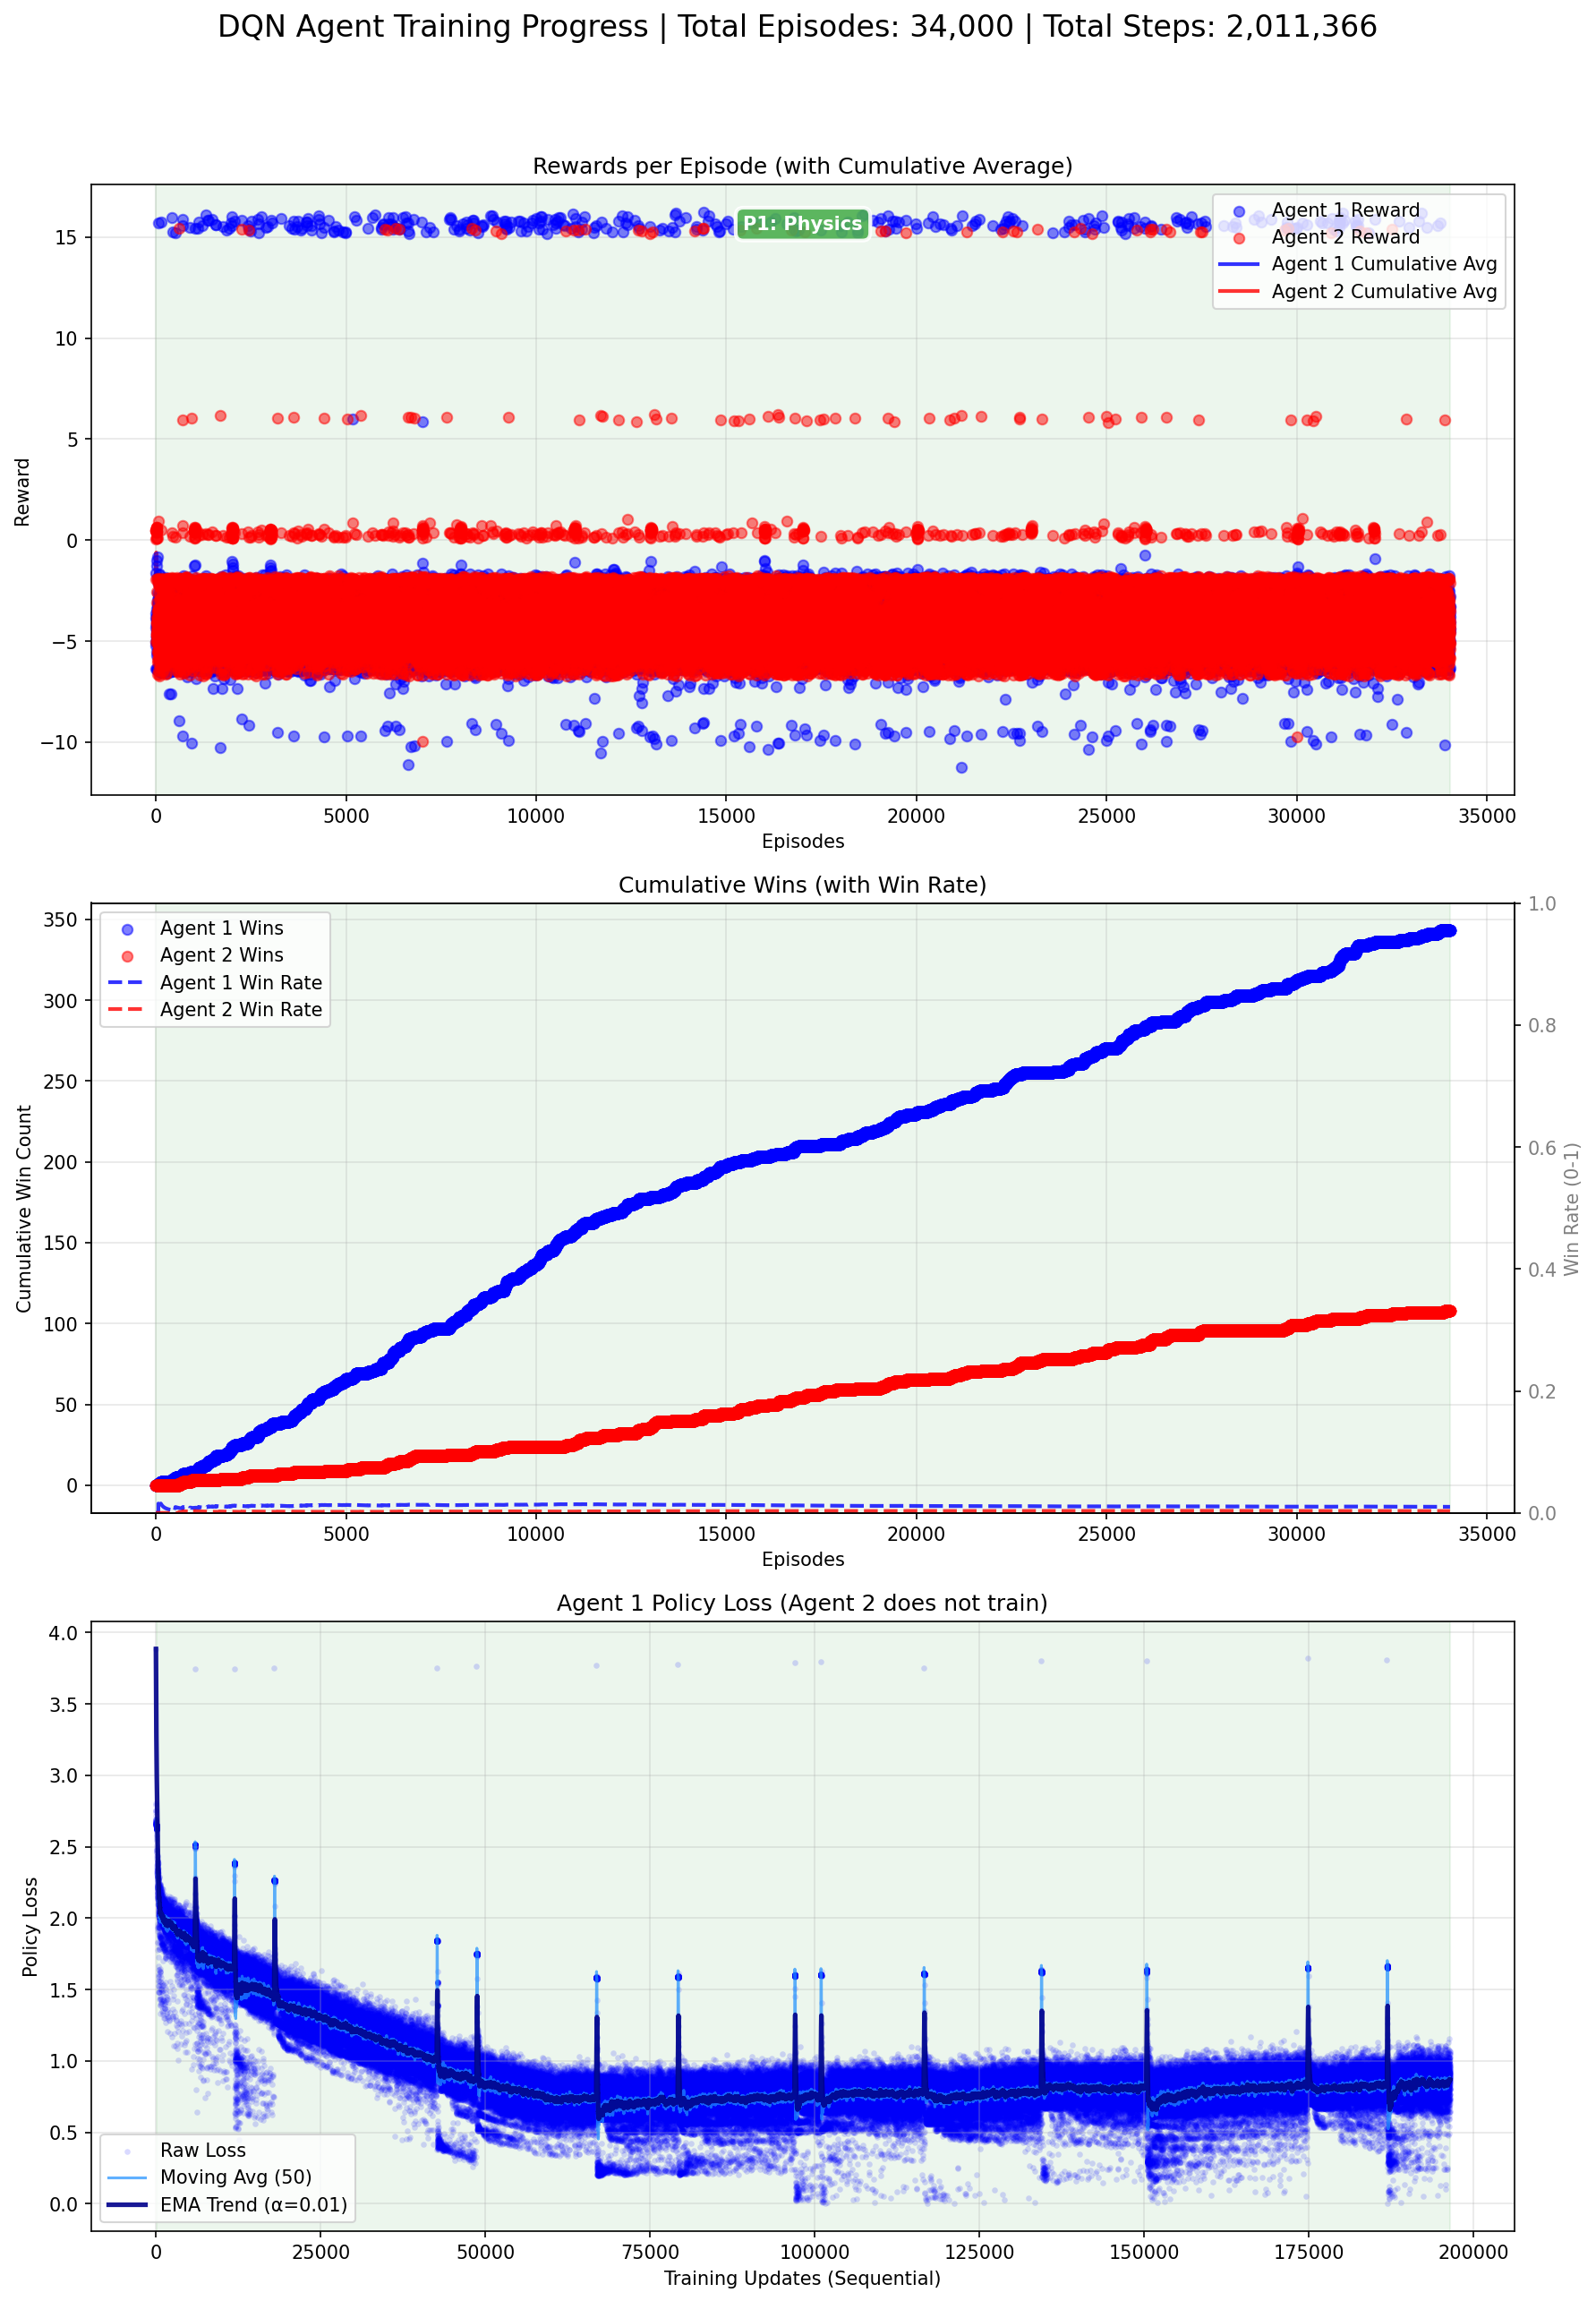
\includegraphics[width=0.9\textwidth,height=0.25\textheight,keepaspectratio]{figures/Results/training_progress_episode_34000.png}
    \caption{Training Progress: Episode 34,000}
    \label{fig:train_34k}
\end{figure}

\section{Discussion on Training Progress and Model Behavior}

The transition from early-stage exploration to the current 34,000-episode milestone reveals significant shifts in how the MARQ agent handles complex strategic interactions.

\subsection{Behavioral Evolution}
In early training (Episodes 0--5,000), the agent exhibited stochastic exploration with a high frequency of illegal move attempts and "indiscriminate charging," where high-value pieces like the Marshal were lost in routine skirmishes. By Episode 15,000, a clear shift towards tactical targeting emerged. The agent began to prioritize the capture of suspected lower-rank pieces while exhibiting defensive withdrawals when facing potential high-rank threats.

At the 34,000-episode mark, the model demonstrates "decisive targeting," specifically identifying and pursuing the opponent's flag once its location is inferred. However, this decisiveness is balanced by a "passive shuffling" tendency in common-value midgame states, where the agent avoids high-risk attacks to preserve material. This results in the observed draw-rate stabilization.

\subsection{Implicit Belief and AAREN Performance}
The Action-Augmented Recurrent Encoder (AAREN) has effectively learned to map action sequences to latent piece identities. As training progressed, the KL divergence between the predicted representation and ground truth revealed that the agent consistently identifies specialized units like Scouts (via multi-square movement) and Miners (via bomb engagement patterns) within 5--10 moves of their initial activity. This implicit deduced knowledge is what allows the Rainbow DQN to make calibrated risk assessments without explicit board information.

\subsection{Impact of Reward Overhaul}
The rescaling of rewards to $\pm 1.0$ for terminal states and the tightening of the C51 support to $[-10, +10]$ significantly improved the resolution of the distributional Q-values. Early training runs used a larger range which led to "clumping" of values, making it difficult for the agent to distinguish between marginally better moves. The current architecture allows for 0.4-unit resolution per atom, enabling the agent to better evaluate subtle positional advantages and territorial control rewards.
